%! TEX program = xelatex

\documentclass{article}
\usepackage[a4paper, margin=3cm]{geometry}
\setlength{\parindent}{0pt}
\setlength{\parskip}{1em}
\usepackage{fontspec}
\setmainfont{Lato}

\usepackage{amsmath,amssymb,amsthm}
%\usepackage{hyperref}
\usepackage{verbatim}
\usepackage{graphicx}
%\usepackage{pgfplots}
%\pgfplotsset{compat=1.16}

\title{}
\author{Mikael Myyrä}
\date{}

\begin{document}

\section*{1.}

\begin{gather*}
  \frac{\partial u(x,t)}{\partial t} - \frac{\partial^2 u(x,t)}{\partial x^2} = 0, \quad x \in (1, 2) \\
  u(1,t) = 0, \quad u(2,t) = 0, \\
  u(x,0) = 8(x-1)(2-x) \\
\end{gather*}

\subsection*{(a)}

Tämä on lämpöyhtälö. Laplacen yhtälö ja aaltoyhtälö ovat paikkaderivaatan
suhteen saman näköisiä, mutta Laplacen yhtälössä ei ole aikaderivaattaa ja
aaltoyhtälössä on ajan toinen derivaatta.

\subsection*{(b)}

Diskretoidaan ensin paikan suhteen laskentapisteissä $u_i, i = 1,\dots,N$
keskeisdifferenssillä:
\[
  \frac{\partial u}{\partial t} - \frac{u_{i-1} - 2u_i + u_{i+1}}{h^2} = 0
\]
Matriisimuodossa
\[
  \frac{\partial u}{\partial t} + \frac{1}{h^2}
  \begin{bmatrix}
    2 & -1 \\
    -1 & 2 & -1 \\
       & \vdots & \vdots & \vdots \\
       & & -1 & 2 & -1 \\
       & & & -1 & 2 \\
  \end{bmatrix}
  \mathbf{u} = 0
\]
\[
  \frac{\partial u}{\partial t} + \mathbf{A}\mathbf{u} = 0.
\]
Crank—Nicolson-menetelmällä aikadiskretoinniksi saadaan
\[
  \frac{\mathbf{u}^{(k+1)} - \mathbf{u}^{(k)}}{\Delta t}
  + \frac{1}{2}\mathbf{A}\mathbf{u}^{(k+1)}
  + \frac{1}{2}\mathbf{A}\mathbf{u}^{(k)} = 0,
\]
josta ratkaistaan $\mathbf{u}^{(k+1)}$:
\begin{align*}
  \mathbf{u}^{(k+1)} - \mathbf{u}^{(k)}
  + \frac{1}{2}\Delta t \mathbf{A}\mathbf{u}^{(k+1)}
  &= -\frac{1}{2}\Delta t \mathbf{A}\mathbf{u}^{(k)} \\
  (\mathbf{I} + \frac{1}{2}\Delta t \mathbf{A})\mathbf{u}^{(k+1)}
  &= (\mathbf{I} - \frac{1}{2}\Delta t \mathbf{A})\mathbf{u}^{(k)} \\
  \mathbf{u}^{(k+1)} &= (\mathbf{I} + \frac{1}{2}\Delta t \mathbf{A})^{-1}
  (\mathbf{I} - \frac{1}{2}\Delta t \mathbf{A})\mathbf{u}^{(k)}
\end{align*}
Homogeeniset Dirichlet-reunaehdot toteutuvat tässä suoraan eivätkä vaadi
erityistä huomiointia.

\subsection*{(c)}

Ratkaisija Matlabilla:

\verbatiminput{exam_1_solve.m}

\subsection*{(d)}

Hilavälillä $\frac{1}{10}$ paikka-askelia on 10, aika-askel on $\frac{1}{200}$
ja askelia tarvitaan 100, jotta päästään ajan hetkeen $\frac{1}{2}$.
Syöttämällä nämä parametrit ratkaisijaan:

\begin{verbatim}
exam_1_solve(10, 1/200, 100)
\end{verbatim}

saadaan tulokseksi
\[
  \begin{bmatrix}
   0.0047718 \\
   0.0090765 \\
   0.0124927 \\
   0.0146861 \\
   0.0154419 \\
   0.0146861 \\
   0.0124927 \\
   0.0090765 \\
   0.0047718 \\
  \end{bmatrix}.
\]

\newpage
\section*{2.}

\subsection*{(a)}

Järjestämällä termejä uudelleen vastaamaan jatkuvan yhtälön muotoa saadaan
\[
  \frac{u^{(k+1)} - u^{(k)}}{\Delta t}
  - \kappa \frac{-\frac{1}{12}u_{j-2}^{(k)} + \frac{4}{3}u_{j-1}^{(k)}
  - \frac{5}{2}u_j^{(k)} + \frac{4}{3}u_{j+1} - \frac{1}{12}u_{j+2}^{(k)}}{h^2} = 0,
\]
mistä nähdään, että aikadiskretointiin on käytetty etenevää differenssiä ja
paikkadiskretointiin vii\-den pisteen kaaviota (luento 6).

\subsection*{(b)}

Tehtävä matriisimuodossa k:nnelle aika-askelelle (homogeenisellä
Dirichlet-reunaehdolla) on
\[
  \mathbf{u}^{(k)} = \Big(\mathbf{I} + \frac{\kappa\Delta t}{h^2}
  \begin{bmatrix}
    -\frac{5}{2} & \frac{4}{3} & -\frac{1}{12} \\
    \frac{4}{3} & -\frac{5}{2} & \frac{4}{3} & -\frac{1}{12} \\
    -\frac{1}{12} & \frac{4}{3} & -\frac{5}{2} & \frac{4}{3} & -\frac{1}{12} \\
                  & \ddots & \ddots & \ddots & \ddots & \ddots \\
                  & & -\frac{1}{12} & \frac{4}{3} & -\frac{5}{2} & \frac{4}{3} & -\frac{1}{12} \\
                  & & & -\frac{1}{12} & \frac{4}{3} & -\frac{5}{2} & \frac{4}{3} \\
                  & & & & -\frac{1}{12} & \frac{4}{3} & -\frac{5}{2} \\
  \end{bmatrix}
  \Big)^k \mathbf{u}^{(0)}.
\]
Jotta menetelmä olisi stabiili, täytyy kerroinmatriisin suurimman ominaisarvon
itseisarvon olla $\leq 1$. Matriisi on symmetrinen pentadiagonaalimatriisi, joten
sen ominaisarvot saadaan tehtävässä annetulla kaavalla, jossa
\[
  a_0 = 1 - \frac{5\kappa\Delta t}{2h^2},
\]
\[
  a_1 = \frac{4\kappa\Delta t}{3h^2}
\]
ja
\[
  a_2 = -\frac{\kappa\Delta t}{12h^2}.
\]
Ominaisarvot ovat siis
\begin{align*}
  \lambda_j &= 1 - \frac{5\kappa\Delta t}{2h^2}
  + 2\Big(\frac{4\kappa\Delta t}{3h^2}\Big) \cos\Big(\frac{j\pi}{N+1}\Big)
  + 2\Big(-\frac{\kappa\Delta t}{12h^2}\Big) \cos\Big(\frac{2j\pi}{N+1}\Big),
  \quad j = 1,2,\dots,N. \\
\end{align*}
$|\lambda_j| \leq 1$, jos
\[
  0 \leq \frac{5\kappa\Delta t}{2h^2}
  - \frac{8\kappa\Delta t}{3h^2} \cos\Big(\frac{j\pi}{N+1}\Big)
  + \frac{\kappa\Delta t}{6h^2} \cos\Big(\frac{2j\pi}{N+1}\Big)
  \leq 2.
\]
Lausekkeen arvo on pienimmillään, kun $j = 1$, jolloin molemmat kosinitermit
lähestyvät 1:tä, kun matriisin koko kasvaa. Rajalla saadaan
\[
  \frac{5\kappa\Delta t}{2h^2} - \frac{8\kappa\Delta t}{3h^2} + \frac{\kappa\Delta t}{6h^2}
  = 0,
\]
joka on aina $\geq 0$ ja $\leq 2$ riippumatta vakioiden arvoista.

Suurimman arvonsa lauseke saa, kun $j = N$, jolloin ensimmäisen kosinin arvo
lähestyy -1:tä ja toisen 1:tä. Tällöin lauseke on
\[
  \frac{5\kappa\Delta t}{2h^2} + \frac{8\kappa\Delta t}{3h^2} - \frac{\kappa\Delta t}{6h^2}
  = \frac{5\kappa \Delta t}{h^2}.
\]
Tämä on aina suurempaa kuin nolla, koska kaikki vakiot ovat positiivisia, joten
ehdoksi jää
\[
  \frac{5\kappa \Delta t}{h^2} \leq 2
  \iff
  \Delta t \leq \frac{2h^2}{5\kappa}.
\]

\newpage
\section*{3.}

\subsection*{(a)}

Tehtävä on epähomogeeninen, ajasta riippumaton toisen asteen
osittaisdifferentiaaliyhtälö äärellisessä tason alueessa epähomogeenisella
Dirichlet-reunaehdolla.  Kurssilla on tutustuttu tällaisten tehtävien
ratkaisuun soveltuviin differenssimenetelmiin ja elementtimenetelmiin,
jälkimmäisistä \\erityisesti Galerkinin menetelmiin. Molemmat menetelmätyypit
selviytyvät epähomogeenisista \\reunaehdoista ja lähdetermistä. Myös suorakulmion
muotoisen alueen diskretointi kummankin menetelmätyypin tarpei\-siin on
helppoa.

\subsection*{(b)}

Stabiilisuus ja tarkkuus ovat aina olennaisia kysymyksiä, koska ne määrittävät,
saadaanko järkevää ratkaisua lainkaan ja miten lähellä todellisuutta se on.
Lisäksi menetelmän kuluttama laskenta-aika voi olla tärkeä erityisesti suurikokoisissa
tehtävissä, jolloin on syytä tarkastella menetelmän aikavaativuutta suhteessa
tarkkuuteen ja stabiilisuuteen. Jos menetelmä täytyy toteuttaa itse, ja varsinkin
jos se täytyy tehdä aikataulussa, voi myös toteutuksen haastavuus olla tärkeä
kysymys.

\subsection*{(c)}

Valitsen tarkasteltavaksi differenssimenetelmän, koska se on ehtinyt tulla
kurssin aikana parhaiten tutuksi.

Tehtävän ratkaiseminen alkaa paikkadiskretointimenetelmän valinnalla.  Tähän
kuuluu differenssiapproksimaation, laskentapisteiden ja niiden indeksoinnin
määrittely. Tyypillinen valinta on keskeisdifferenssi ja koordinaattiakselien
suuntainen laskentahila, jossa indeksointi tapahtuu vasemmalta oikealle ja
alhaalta ylös. Tässä tehtävässä ei ole aikariippuvuutta, joten aikadiskretointia
ei tarvita.

Differenssiapproksimaation valinta ja hilan tiheys vaikuttavat
menetelmän tarkkuuteen ja aikavaativuuteen. Tarkemmat
differenssiapproksimaatiot vaativat enemmän laskutoimituksia ja mahdolli\-sesti
myös lisälaskentapisteitä alueen ulkopuolelta, mikä monimutkaistaa tehtävän
muodostamista. Mitä lähempänä toisiaan laskentapisteet ovat, sitä tarkempi on
lopputulos, mutta sitä useammissa pisteissä joudutaan suorittamaan laskentaa
koko alueen kattamiseksi.  Jokainen laskentapiste vie myös tietyn määrän tilaa
muistissa.

Seuraavaksi valitulla differenssiapproksimaatiolla muodostetaan diskreetti
tehtävä jokaisessa las\-kentapisteessä. Näistä muodostuu yhtälöryhmä, joka
voidaan esittää matriisiyhtälönä $\mathbf{A}\mathbf{u} = \mathbf{b}$, missä
$\mathbf{u}$ on laskentapisteet sisältävä tuntematon vektori ja $\mathbf{b}$
sisältää lähdetermin arvot laskentapisteissä. Tässä tapauksessa $\mathbf{u}$ ei
sisällä alueen reunapisteitä. Yhtälöryhmään kuuluvat myös reuna\-ehdot, jotka
voidaan tässä tapauksessa yhdistää vektoriin $\mathbf{b}$. Muun tyyppiset
reunaehdot saattavat tuottaa yhtälöitä, jotka täytyy lisätä uusina riveinä
matriiseihin.

Kun tehtävä on saatu matriisimuotoon, tarvitaan jokin menetelmä käänteismatriisin
laskemiseen, jotta saadaan ratkaisu $\mathbf{u} = \mathbf{A}^{-1}\mathbf{b}$.
Tähän voidaan käyttää suoria menetelmiä, kuten LU-hajotelmaa, tai iteratiivisia
menetelmiä, kuten Gauss—Seidel- tai Jacobi-iteraatiota. Tässäkin menetelmän
va\-linta vaikuttaa aika- ja tilavaativuuteen. Usein matriisi $\mathbf{A}$ on
symmetrinen nauhamatriisi, johon voidaan käyttää tehokkaampia menetelmiä
kuin yleisiin matriiseihin.

\newpage
\section*{5.}

\subsection*{(a)}

\[
  -\Delta u(x_1,x_2) = f(x_1,x_2)
\]

Olkoon $v$ mikä tahansa jatkuva funktio, joka toteuttaa tehtävän reunaehdon
$v(x_1,x_2) = 0$ ja jonka derivaatat ovat neliöintegroituvia. Kerrotaan yhtälö
$v$:llä ja integroidaan alueen $\Omega$ yli:
\[
  -\int_{\Omega} (\nabla \cdot \nabla)uv\,dx = \int_{\Omega} fv\,dx
\]
Greenin lause:
\[
  \int_{\Omega} \nabla v \cdot \nabla u\,dx
  - \int_{\partial \Omega} v\frac{\partial u}{\partial \mathbf{n}}\,dx
  = \int_{\Omega} fv\,dx
\]
Reunalla on kaikkialla ehto $u,v=0$, joten reunan käyräintegraali häviää.
\[
  \int_{\Omega} \nabla v \cdot \nabla u\,dx = \int_{\Omega} fv\,dx
\]
Tämä on haluttu heikko muoto.

\subsection*{(b)}

\subsubsection*{i.}

\verb#verkko.m#-tiedostossa määritellään aloitusverkko, jota tihentämällä
lopullinen laskentaverkko muodostetaan. Siis sen reunat ovat laskenta-alueen
reunat. Verkko kattaa neliöalueen $(0, 1) \times (0, 1)$.

Lähdetermi määritellään rivillä
\begin{verbatim}
  funktio=(3*x1+x1^2)*exp(x1)*x2*(1-x2) + 2*x1*(1-x1)*exp(x1);
\end{verbatim}
joka on matematiikan notaatiolla kirjoitettuna
\[
  f(x_1,x_2) = (3x_1 + x_1^2)e^{x_2}(1-x_2) + 2x^1(1-x_1)e^{x_1}.
\]

\subsubsection*{ii.}

Yhdeksän solmun verkko muodostuu yhden tihennyksen jälkeen.
Ohjelman tulosteen
\begin{verbatim}
solmut =

   0.00000   0.00000   1.00000
   1.00000   0.00000   1.00000
   1.00000   1.00000   1.00000
   0.00000   1.00000   1.00000
   0.50000   0.00000   1.00000
   1.00000   0.50000   1.00000
   0.50000   0.50000   0.00000
   0.50000   1.00000   1.00000
   0.00000   0.50000   1.00000

elementit =

   1   5   7
   2   6   5
   3   7   6
   5   6   7
   1   7   9
   3   8   7
   4   9   8
   7   8   9
\end{verbatim}
järjestyksestä nähdään solmujen ja elementtien numerointi.
Kuva:

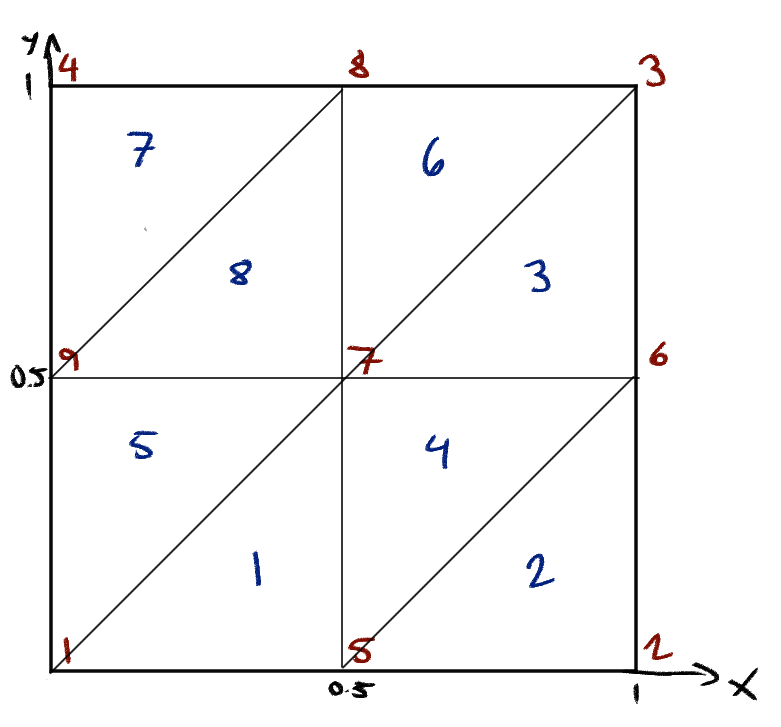
\includegraphics[width=250pt]{exam_5_ii.jpg}

Solmut on numeroitu punaisella ja elementit sinisellä.

Numerointi on erilainen kuin luentoesimerkissä. Tässä solmupisteiden indeksit
pysyvät samoina, kun verkkoa tihennetään, ja vain väleihin tulevat uudet pisteet
saavat uudet indeksit.

\subsubsection*{iii.}

Jouduin muokkaamaan ratkaisijaa sen verran, että vaihdoin
\verb#sparse#-matriisin tilalle tavallisen \verb#zeros#-matriisin, koska
käyttöjärjestelmäni Octave-paketista puuttuu harvojen matriisien käsittelyyn
tarvittava kirjasto. Tämän ei pitäisi vaikuttaa oleellisesti virheeseen.

Saan seuraavanlaisia arvoja suurimmalle virheelle ja energianormille,
kun kasvatan tihennyskerroin-muuttujan arvoa:

\begin{tabular}{ c c c }
  tihennyskerroin & max(virhe) & energianormi \\
  \hline
  1 & 0.019812 & 0.039623 \\
  2 & 0.0064817 & 0.016129 \\
  3 & 0.0018156 & 0.0045704 \\
  4 & 0.00046901 & 0.0011807 \\
  5 & 0.00011765 & 0.00029768 \\
\end{tabular}

Virhe pienenee joka kerta hilavälin pienentyessä, joten näyttää hyvin
todennäköiseltä, että menetel\-mä suppenee. 

Tihennyskertoimen kasvattaminen yhdellä puolittaa laskentapisteiden välimatkan.
Jos suppenemisnopeus olisi suoraan verrannollinen pisteiden välimatkoihin, niin
myös virheen pitäisi tällöin puolittua. Tämän otoksen perusteella vaikuttaa
siltä, että virhe pienenee tätä nopeammin ja lisäksi muutos nopeutuu, kun väli
pienenee. Arvioisin, että virhe on verrannollinen välin pituuden neliöön.

\end{document}
